% Options for packages loaded elsewhere
\PassOptionsToPackage{unicode}{hyperref}
\PassOptionsToPackage{hyphens}{url}
%
\documentclass[
]{article}
\usepackage{lmodern}
\usepackage{amssymb,amsmath}
\usepackage{ifxetex,ifluatex}
\ifnum 0\ifxetex 1\fi\ifluatex 1\fi=0 % if pdftex
  \usepackage[T1]{fontenc}
  \usepackage[utf8]{inputenc}
  \usepackage{textcomp} % provide euro and other symbols
\else % if luatex or xetex
  \usepackage{unicode-math}
  \defaultfontfeatures{Scale=MatchLowercase}
  \defaultfontfeatures[\rmfamily]{Ligatures=TeX,Scale=1}
\fi
% Use upquote if available, for straight quotes in verbatim environments
\IfFileExists{upquote.sty}{\usepackage{upquote}}{}
\IfFileExists{microtype.sty}{% use microtype if available
  \usepackage[]{microtype}
  \UseMicrotypeSet[protrusion]{basicmath} % disable protrusion for tt fonts
}{}
\makeatletter
\@ifundefined{KOMAClassName}{% if non-KOMA class
  \IfFileExists{parskip.sty}{%
    \usepackage{parskip}
  }{% else
    \setlength{\parindent}{0pt}
    \setlength{\parskip}{6pt plus 2pt minus 1pt}}
}{% if KOMA class
  \KOMAoptions{parskip=half}}
\makeatother
\usepackage{xcolor}
\IfFileExists{xurl.sty}{\usepackage{xurl}}{} % add URL line breaks if available
\IfFileExists{bookmark.sty}{\usepackage{bookmark}}{\usepackage{hyperref}}
\hypersetup{
  pdftitle={Introduction to Bayesian linear regression with brms --- Part III},
  pdfauthor={Stefano Coretta},
  hidelinks,
  pdfcreator={LaTeX via pandoc}}
\urlstyle{same} % disable monospaced font for URLs
\usepackage[margin=1in]{geometry}
\usepackage{color}
\usepackage{fancyvrb}
\newcommand{\VerbBar}{|}
\newcommand{\VERB}{\Verb[commandchars=\\\{\}]}
\DefineVerbatimEnvironment{Highlighting}{Verbatim}{commandchars=\\\{\}}
% Add ',fontsize=\small' for more characters per line
\usepackage{framed}
\definecolor{shadecolor}{RGB}{248,248,248}
\newenvironment{Shaded}{\begin{snugshade}}{\end{snugshade}}
\newcommand{\AlertTok}[1]{\textcolor[rgb]{0.94,0.16,0.16}{#1}}
\newcommand{\AnnotationTok}[1]{\textcolor[rgb]{0.56,0.35,0.01}{\textbf{\textit{#1}}}}
\newcommand{\AttributeTok}[1]{\textcolor[rgb]{0.77,0.63,0.00}{#1}}
\newcommand{\BaseNTok}[1]{\textcolor[rgb]{0.00,0.00,0.81}{#1}}
\newcommand{\BuiltInTok}[1]{#1}
\newcommand{\CharTok}[1]{\textcolor[rgb]{0.31,0.60,0.02}{#1}}
\newcommand{\CommentTok}[1]{\textcolor[rgb]{0.56,0.35,0.01}{\textit{#1}}}
\newcommand{\CommentVarTok}[1]{\textcolor[rgb]{0.56,0.35,0.01}{\textbf{\textit{#1}}}}
\newcommand{\ConstantTok}[1]{\textcolor[rgb]{0.00,0.00,0.00}{#1}}
\newcommand{\ControlFlowTok}[1]{\textcolor[rgb]{0.13,0.29,0.53}{\textbf{#1}}}
\newcommand{\DataTypeTok}[1]{\textcolor[rgb]{0.13,0.29,0.53}{#1}}
\newcommand{\DecValTok}[1]{\textcolor[rgb]{0.00,0.00,0.81}{#1}}
\newcommand{\DocumentationTok}[1]{\textcolor[rgb]{0.56,0.35,0.01}{\textbf{\textit{#1}}}}
\newcommand{\ErrorTok}[1]{\textcolor[rgb]{0.64,0.00,0.00}{\textbf{#1}}}
\newcommand{\ExtensionTok}[1]{#1}
\newcommand{\FloatTok}[1]{\textcolor[rgb]{0.00,0.00,0.81}{#1}}
\newcommand{\FunctionTok}[1]{\textcolor[rgb]{0.00,0.00,0.00}{#1}}
\newcommand{\ImportTok}[1]{#1}
\newcommand{\InformationTok}[1]{\textcolor[rgb]{0.56,0.35,0.01}{\textbf{\textit{#1}}}}
\newcommand{\KeywordTok}[1]{\textcolor[rgb]{0.13,0.29,0.53}{\textbf{#1}}}
\newcommand{\NormalTok}[1]{#1}
\newcommand{\OperatorTok}[1]{\textcolor[rgb]{0.81,0.36,0.00}{\textbf{#1}}}
\newcommand{\OtherTok}[1]{\textcolor[rgb]{0.56,0.35,0.01}{#1}}
\newcommand{\PreprocessorTok}[1]{\textcolor[rgb]{0.56,0.35,0.01}{\textit{#1}}}
\newcommand{\RegionMarkerTok}[1]{#1}
\newcommand{\SpecialCharTok}[1]{\textcolor[rgb]{0.00,0.00,0.00}{#1}}
\newcommand{\SpecialStringTok}[1]{\textcolor[rgb]{0.31,0.60,0.02}{#1}}
\newcommand{\StringTok}[1]{\textcolor[rgb]{0.31,0.60,0.02}{#1}}
\newcommand{\VariableTok}[1]{\textcolor[rgb]{0.00,0.00,0.00}{#1}}
\newcommand{\VerbatimStringTok}[1]{\textcolor[rgb]{0.31,0.60,0.02}{#1}}
\newcommand{\WarningTok}[1]{\textcolor[rgb]{0.56,0.35,0.01}{\textbf{\textit{#1}}}}
\usepackage{graphicx}
\makeatletter
\def\maxwidth{\ifdim\Gin@nat@width>\linewidth\linewidth\else\Gin@nat@width\fi}
\def\maxheight{\ifdim\Gin@nat@height>\textheight\textheight\else\Gin@nat@height\fi}
\makeatother
% Scale images if necessary, so that they will not overflow the page
% margins by default, and it is still possible to overwrite the defaults
% using explicit options in \includegraphics[width, height, ...]{}
\setkeys{Gin}{width=\maxwidth,height=\maxheight,keepaspectratio}
% Set default figure placement to htbp
\makeatletter
\def\fps@figure{htbp}
\makeatother
\setlength{\emergencystretch}{3em} % prevent overfull lines
\providecommand{\tightlist}{%
  \setlength{\itemsep}{0pt}\setlength{\parskip}{0pt}}
\setcounter{secnumdepth}{5}
\ifluatex
  \usepackage{selnolig}  % disable illegal ligatures
\fi

\title{Introduction to Bayesian linear regression with brms --- Part
III}
\author{Stefano Coretta}
\date{26/06/2020}

\begin{document}
\maketitle

{
\setcounter{tocdepth}{2}
\tableofcontents
}
\begin{Shaded}
\begin{Highlighting}[]
\NormalTok{pilot \textless{}{-}}\StringTok{ }\KeywordTok{list.files}\NormalTok{(}
  \DataTypeTok{path =} \StringTok{"./data/perceptual/"}\NormalTok{,}
  \DataTypeTok{pattern =} \StringTok{"*.csv"}\NormalTok{,}
  \DataTypeTok{full.names =} \OtherTok{TRUE}
\NormalTok{) }\OperatorTok{\%\textgreater{}\%}
\StringTok{  }\KeywordTok{map\_df}\NormalTok{(}\OperatorTok{\textasciitilde{}}\KeywordTok{read\_csv}\NormalTok{(., }\DataTypeTok{col\_types =} \KeywordTok{cols}\NormalTok{(}\DataTypeTok{.default =} \StringTok{"c"}\NormalTok{))) }\OperatorTok{\%\textgreater{}\%}
\StringTok{  }\KeywordTok{mutate}\NormalTok{(}
    \DataTypeTok{key\_resp\_2.keys =} \KeywordTok{ifelse}\NormalTok{(key\_resp\_}\FloatTok{2.}\NormalTok{keys }\OperatorTok{==}\StringTok{ "z"}\NormalTok{, }\StringTok{"d"}\NormalTok{, }\StringTok{"t"}\NormalTok{),}
    \DataTypeTok{key\_resp\_8.keys =} \KeywordTok{ifelse}\NormalTok{(key\_resp\_}\FloatTok{8.}\NormalTok{keys }\OperatorTok{==}\StringTok{ "z"}\NormalTok{, }\StringTok{"t"}\NormalTok{, }\StringTok{"d"}\NormalTok{),}
    \DataTypeTok{response =} \KeywordTok{coalesce}\NormalTok{(key\_resp\_}\FloatTok{2.}\NormalTok{keys, key\_resp\_}\FloatTok{8.}\NormalTok{keys),}
    \DataTypeTok{response =} \KeywordTok{factor}\NormalTok{(response, }\DataTypeTok{levels =} \KeywordTok{c}\NormalTok{(}\StringTok{"d"}\NormalTok{, }\StringTok{"t"}\NormalTok{)),}
    \DataTypeTok{burst =} \KeywordTok{as.numeric}\NormalTok{(burst),}
    \DataTypeTok{voicing =} \KeywordTok{as.numeric}\NormalTok{(voicing),}
    \DataTypeTok{response\_n =} \KeywordTok{as.numeric}\NormalTok{(response) }\OperatorTok{{-}}\StringTok{ }\DecValTok{1}\NormalTok{,}
    \DataTypeTok{vowel =} \KeywordTok{factor}\NormalTok{(vowel, }\DataTypeTok{levels =} \KeywordTok{c}\NormalTok{(}\StringTok{"a"}\NormalTok{, }\StringTok{"i"}\NormalTok{, }\StringTok{"u"}\NormalTok{))}
\NormalTok{  ) }\OperatorTok{\%\textgreater{}\%}
\StringTok{  }\KeywordTok{filter}\NormalTok{(}\OperatorTok{!}\KeywordTok{is.na}\NormalTok{(response))}

\KeywordTok{contrasts}\NormalTok{(pilot}\OperatorTok{$}\NormalTok{vowel) \textless{}{-}}\StringTok{ "contr.sum"}

\NormalTok{burst \textless{}{-}}\StringTok{ }\KeywordTok{filter}\NormalTok{(pilot, condition }\OperatorTok{==}\StringTok{ "burst"}\NormalTok{) }\OperatorTok{\%\textgreater{}\%}
\StringTok{  }\KeywordTok{select}\NormalTok{(burst, vowel, participant, response, response\_n)}
\NormalTok{voicing \textless{}{-}}\StringTok{ }\KeywordTok{filter}\NormalTok{(pilot, condition }\OperatorTok{==}\StringTok{ "voicing"}\NormalTok{)}
\end{Highlighting}
\end{Shaded}

\hypertarget{quick-recap}{%
\section{Quick recap}\label{quick-recap}}

We collect a sample of observations \(y = (y_1, ..., y_n)\) generated by
a \textbf{random variable} \(Y\), i.e.~we sample values generated by a
random event.

We use the sample \(y\) to obtain an estimate of \(Y\), i.e.~we perform
statistical inference.

\(Y\) is both \emph{unknown} (we don't know the value it takes) and
\emph{uncertain} (we can't be sure about the value it takes).
Uncertainty can be expressed by probability distributions.

A \textbf{probability distribution} is a list of values along with its
corresponding probability. Probabilities take on values between 0
(impossible event) and 1 (certain event).

Probability distributions can be summarised using \textbf{parameters}.
The \emph{normal distribution} (aka Gaussian distribution) has two
parameters: the mean \(\mu\) and the standard deviation \(\sigma\) (or
the variance \(\sigma^2\)). Parameters are random variables themselves,
i.e.~they are uncertain. We can express distribution parameters with
probability distributions (which have \emph{hyperparameters}, or in
other words parameters on parameters). We can estimate the
hyperparameters from the sample \(y\).

For example:

\[ y_i \sim Normal(\mu, \sigma) \] \[ \mu \sim Normal(\mu_1, \sigma_1)\]
\[ \sigma \sim HalfCauchy(x_0, \gamma)\]

\(y\) is our outcome variable (our sample of values). We believe that
the values of \(y\) were generated by a normal distribution which has
parameters \(\mu\) and \(\sigma\) (this is the \emph{likelihood}, or
simply the \emph{probability distribution of the outcome variable}). We
believe that the value of \(\mu\) comes from a normal distribution with
\(\mu_1\) and \(\sigma_1\) and that the value of \(\sigma\) comes from a
half Cauchy distribution with parameters \(x_0\) and \(\gamma\).

We convey our prior beliefs of what \(\mu\) and \(\sigma\) might be by
specifying probability distributions (the \textbf{prior probability
distributions}, or \emph{priors}). In other words, we specify the
hyperparameters \(\mu_1\), \(\sigma_1\), \(x_0\), \(\gamma\).

These hyperparameters are updated by the Bayesian model with the
information provided by the sample, and we thus obtain the
\textbf{posterior probability distributions} (or \emph{posteriors}) of
\(\mu\) and \(\sigma\).

\hypertarget{discrete-variables}{%
\section{Discrete variables}\label{discrete-variables}}

In Part I and II we focussed on \emph{continuous variables} and
continous probability distributions, among which the normal (Gaussian)
distribution is the most commonly employed for statistical analyses. A
continuous variable is a variable that can take on any value between two
specific values (numbers). For example, height, weight, vowel formants,
segment duration, and reaction times are all continuous variables.

Some events, on the other hand, generate \textbf{discrete variables},
i.e.~variables that can only take specific values and not values in
between. For example, binary outcomes like flips of a coin, yes/no
questions, and success/failure are all discrete variables. Counts are
discrete as well (if you count how many fish there are in a pond, you
can't have 5.5 fish).

Probability distributions that generate discrete variables are discrete
probability distributions.

In this tutorial, I will discuss how to model binary outcomes using
binomial/Bernoulli distributions.

\hypertarget{binary-outcomes-binomialbernoulli}{%
\section{Binary outcomes:
binomial/Bernoulli}\label{binary-outcomes-binomialbernoulli}}

Binary outcomes (yes/no questions, binary choices, successes/failures)
follow the \textbf{binomial distribution}. The binomial distribution has
two parameters: the number of trials \(n\) and the probability \(p\) of
getting one of the two oucomes in each trial (\(p\) = probability of
getting A, \(1 - p\) = probability of getting B).

When fitting a model with the binomial family, the data needs to be in a
special format. Let's assume you asked a yes/no question and
participants answered either ``yes'' (= 1) or ``no'' (= 0). You have to
indicate the total number of trials (for example, 20 participants), and
the number of trials in which the participants have answered ``yes'' (=
1). For example, 15/20 participants have answered ``yes''.

However, binary outcome variables can also be formalised through the
\textbf{Bernoulli distribution}. The Bernoulli distribution is a special
case of the binomial, where the total number of trials \(n\) is 1, and
\(p\) is the probability of one of the two oucomes (for example,
``yes'', 1). With the Bernoulli distribution, the data is generally
entered as we normally do, i.e.~for each observation we state whether
the answer was 0 or 1 (``yes'' or ``no'', etc\ldots). In this format, we
don't have to specify the total number of trials.

If you used \texttt{glm{[}er{]}()} with \texttt{family\ =\ binomial}
before, note that the model automatically uses the Bernoulli
distribution when you don't specify the total number of trials and the
data is in the ``long'' format (one trial per row, specifying what the
outcome was). On the other hand, \texttt{brms()} does not do this, so
you have to explicitly use the \texttt{bernoulli()} family when you want
to fit ``binomial regressions''.

\hypertarget{example-perception-of-voicing-in-italian}{%
\section{Example: perception of voicing in
Italian}\label{example-perception-of-voicing-in-italian}}

To show hot to fit a binomial/Bernoulli regression, we will use data
from a pilot study of the perception of voicing in Italian stops (note
that the design of the experiment was very limited, so take this as toy
data).

In this pilot study, I asked listeners to say whether they heard a
voiced or a voiced stop after listening to synthetic nonce words
(\emph{pata}, \emph{piti}, \emph{putu}). The duration of the burst of
the /t/ was manipulated in 5 steps (details don't matter), where 0 was
the shorter duration and 5 the longest (so a total of 6 degrees of
duration). The /t/ was voiceless throughout its closure in all tokens.

Here is how the data frame looks like (\texttt{burst} is the burst
duration step between 0 and 5, and \texttt{response} is the listener
response, either voiced ``d'' or voiceless ``t''):

\begin{Shaded}
\begin{Highlighting}[]
\NormalTok{burst}
\end{Highlighting}
\end{Shaded}

\begin{verbatim}
## # A tibble: 360 x 5
##    burst vowel participant response response_n
##    <dbl> <fct> <chr>       <fct>         <dbl>
##  1     3 u     f001        t                 1
##  2     2 u     f001        d                 0
##  3     4 u     f001        t                 1
##  4     0 a     f001        d                 0
##  5     1 u     f001        t                 1
##  6     5 i     f001        t                 1
##  7     2 a     f001        t                 1
##  8     3 a     f001        t                 1
##  9     3 i     f001        t                 1
## 10     1 a     f001        d                 0
## # ... with 350 more rows
\end{verbatim}

What we want to model here is the probability of choosing ``voiceless''
with increasing burst duration.

We can fit a Bernoulli distribution to the outcome variable
(\texttt{response}) since it's binary (``voiceless'' or ``voiced''). The
code of a simple model for the binary outcome \texttt{response} looks
like this:

\begin{Shaded}
\begin{Highlighting}[]
\KeywordTok{brm}\NormalTok{(}
\NormalTok{  response }\OperatorTok{\textasciitilde{}}
\StringTok{    }\NormalTok{burst }\OperatorTok{+}
\StringTok{    }\NormalTok{(burst }\OperatorTok{|}\StringTok{ }\NormalTok{participant),}
  \DataTypeTok{data =}\NormalTok{ burst,}
  \DataTypeTok{family =} \KeywordTok{bernoulli}\NormalTok{()}
\NormalTok{)}
\end{Highlighting}
\end{Shaded}

As usual, the first thing is to set up our priors. Let's check which
ones we need to specify.

\begin{Shaded}
\begin{Highlighting}[]
\KeywordTok{get\_prior}\NormalTok{(}
\NormalTok{  response }\OperatorTok{\textasciitilde{}}
\StringTok{    }\NormalTok{burst }\OperatorTok{+}
\StringTok{    }\NormalTok{(burst }\OperatorTok{|}\StringTok{ }\NormalTok{participant),}
  \DataTypeTok{data =}\NormalTok{ burst,}
  \DataTypeTok{family =} \KeywordTok{bernoulli}\NormalTok{()}
\NormalTok{)}
\end{Highlighting}
\end{Shaded}

\begin{verbatim}
##                  prior     class      coef       group resp dpar nlpar bound
## 1                              b                                            
## 2                              b     burst                                  
## 3               lkj(1)       cor                                            
## 4                            cor           participant                      
## 5 student_t(3, 0, 2.5) Intercept                                            
## 6 student_t(3, 0, 2.5)        sd                                            
## 7                             sd           participant                      
## 8                             sd     burst participant                      
## 9                             sd Intercept participant
\end{verbatim}

So, nothing unusual. There's an \texttt{Intercept}, \texttt{b} for
burst, \texttt{cor} because we included a random slope, and \texttt{sd}
for the random intercept.

There's a catch though. Since what we are modelling here is a
probability, which is a number between 0 and 1, we have to use a ``link
function'' that maps (transforms) the numbers between 0 and 1 of the
outcome variable to a continuous scale of unbounded numbers. These
numbers on a continuous scale are used to estimate the coefficients of
the model. (I won't explain link functions in details, and you might be
familiar with the concept already if you fitted binomial regressions
before).

The link function of Bernoulli models is the logistic unit function, or
``logit'' function for short (the link function for Gaussian/normal
models is the ``identity'' function, which means that the outcome
variable is not transformed). When using the logit function, the
coefficients returned by the model are in log-odds, not probabilities.
So priors need to be specified on that same scale, namely log-odds,
which makes things a bit less straightforward.

\hypertarget{priors-for-models-using-bernoulli-distributions}{%
\subsubsection{Priors for models using Bernoulli
distributions}\label{priors-for-models-using-bernoulli-distributions}}

Priors for models that use the Bernoulli distribution for the outcome
variable have to be defined on the log-odd scale. It is thus helpful to
know how percentages (numbers between 0 and 1) map onto log-odds.

The following plot shows percentages on the \emph{x}-axis and the
corresponding log-odds on the \emph{y}-axis. You will notice that a 50\%
probability (\(p = 0.5\)) corresponds to a log-odd of 0. Probabilities
smaller than 0.5 map onto negative log-odds, while probabilities greater
than 0.5 map onto positive log-odds. Finally, when approaching
probabilities 0 and 1, the change in log-odds decreases asymptotically
(ad infinitum), so that most of the variation in log-odds is within the
range -7 and +7. Since log-odds increase/decrease asymptotically, they
are on a continuous scale and can be used in a regression model.

\begin{Shaded}
\begin{Highlighting}[]
\KeywordTok{tibble}\NormalTok{(}
  \DataTypeTok{p =} \KeywordTok{seq}\NormalTok{(}\DecValTok{0}\NormalTok{, }\DecValTok{1}\NormalTok{, }\DataTypeTok{by =} \FloatTok{0.001}\NormalTok{),}
  \DataTypeTok{log\_odds =} \KeywordTok{qlogis}\NormalTok{(p)}
\NormalTok{) }\OperatorTok{\%\textgreater{}\%}
\StringTok{  }\KeywordTok{ggplot}\NormalTok{(}\KeywordTok{aes}\NormalTok{(p, log\_odds)) }\OperatorTok{+}
\StringTok{  }\KeywordTok{geom\_hline}\NormalTok{(}\KeywordTok{aes}\NormalTok{(}\DataTypeTok{yintercept =} \DecValTok{0}\NormalTok{), }\DataTypeTok{alpha =} \FloatTok{0.5}\NormalTok{) }\OperatorTok{+}
\StringTok{  }\KeywordTok{geom\_line}\NormalTok{() }\OperatorTok{+}
\StringTok{  }\KeywordTok{scale\_y\_continuous}\NormalTok{(}\DataTypeTok{breaks =} \KeywordTok{seq}\NormalTok{(}\OperatorTok{{-}}\DecValTok{6}\NormalTok{, }\DecValTok{6}\NormalTok{, }\DataTypeTok{by =} \DecValTok{2}\NormalTok{)) }\OperatorTok{+}
\StringTok{  }\KeywordTok{labs}\NormalTok{(}
    \DataTypeTok{title =} \StringTok{"Correspondence between probabilities and log{-}odds"}\NormalTok{,}
    \DataTypeTok{x =} \StringTok{"probability"}\NormalTok{,}
    \DataTypeTok{y =} \StringTok{"log{-}odds"}
\NormalTok{  )}
\end{Highlighting}
\end{Shaded}

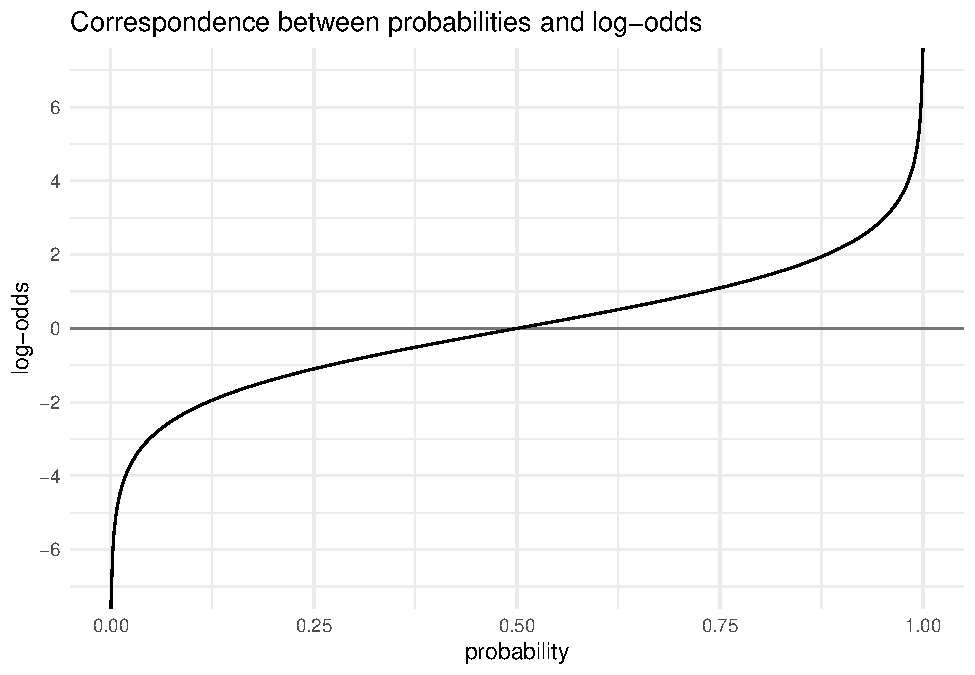
\includegraphics{bayes-reg-3_files/figure-latex/p-log-odds-1.pdf} A
quick way to know which log-odd corresponds to which probability (and
vice versa) is to use the functions \texttt{plogis()} and
\texttt{qlogis()} (\texttt{logis} stands for ``logistic function'').

\begin{Shaded}
\begin{Highlighting}[]
\CommentTok{\# log{-}odds = 0; get probability}
\KeywordTok{plogis}\NormalTok{(}\DecValTok{0}\NormalTok{)}
\end{Highlighting}
\end{Shaded}

\begin{verbatim}
## [1] 0.5
\end{verbatim}

\begin{Shaded}
\begin{Highlighting}[]
\CommentTok{\# p = 0.5; get log{-}odds}
\KeywordTok{qlogis}\NormalTok{(}\FloatTok{0.5}\NormalTok{)}
\end{Highlighting}
\end{Shaded}

\begin{verbatim}
## [1] 0
\end{verbatim}

I suggest playing with these two functions to familiarise yourself
better with the logit function.

We can start now with the prior for the intercept of our model of
voicing perception. In our model, the intercept is the probability of
obtaining a ``voiceless'' response when the burst duration is 0. A very
weakly informative prior would be one which includes the whole range of
probabilities, but in which a probability of 0 or 1 are less likely than
probabilities around 0.5. Such prior can be expressed by a normal
distribution with mean 0 and standard deviation 5
(\texttt{normal(0,\ 5)}).

To see why, we can do our usual maths to get the 95\% credible interval:
mean - 2 times the standard deviation = 0 - 2 x 5 = -10, mean + 2 times
the standard deviation = 0 + 2 * 5 = +10. So, the 95\% credible interval
for \texttt{normal(0,\ 5)} is {[}-10, +10{]}. This interval is in
log-odds and to get the respective probabilities we can use the
\texttt{plogis()} function.

\begin{Shaded}
\begin{Highlighting}[]
\KeywordTok{plogis}\NormalTok{(}\OperatorTok{{-}}\DecValTok{10}\NormalTok{)}
\end{Highlighting}
\end{Shaded}

\begin{verbatim}
## [1] 4.539787e-05
\end{verbatim}

\begin{Shaded}
\begin{Highlighting}[]
\KeywordTok{plogis}\NormalTok{(}\DecValTok{10}\NormalTok{)}
\end{Highlighting}
\end{Shaded}

\begin{verbatim}
## [1] 0.9999546
\end{verbatim}

The output shows that a log-odd of -10 corresponds approximately to a
probability of 0.000045, while a log-odd of 10 corresponds almost to a
probability of 1. In sum, a \texttt{normal(0,\ 5)} prior corresponds to
a belief that the probability of obtaining a ``voiceless'' response when
the burst duration is 0 is anything between 0 and 1 at 95\% confidence.
This is a very weakly informative prior (anything goes).

Now, for the prior of the effect of \texttt{burst} we can use the prior
\texttt{normal(0,\ 2.5)}. The 95\% CI of this prior is {[}-5, +5{]}.
Since \texttt{burst} is a numeric variable, the effect of \texttt{burst}
on the probability of getting a ``voiceless'' response is based on the
unit increase of \texttt{burst}, which means that the effect of
\texttt{burst} tells us what is the change in probability when
increasing the duration of the burst by 1 unit relative to the
intercept. Probabilities can also be expressed in odds and the change in
probability can be expressed as change in odds.

Odds (or odd-ratios) can be calculated from log-odds by exponentiating
the log-odds with the \texttt{exp()} function (this will come handy when
we'll look at Poisson models). For example, a log-odd of 0 corresponds
to an odd of 1 (\(exp(0) = 1\)), i.e.~there is no change. A log-odd of 5
is 148 in odds, meaning that there is an increase in odds by a magnitude
of 148, which is quite a big effect. So a \texttt{normal(0,\ 2.5)} prior
is a very weakly informative prior.

\hypertarget{bernoulli-model}{%
\subsection{Bernoulli model}\label{bernoulli-model}}

We can now define our priors (we would also normally run prior
predictive checks, but I will skip it here to save time).

\begin{Shaded}
\begin{Highlighting}[]
\NormalTok{priors \textless{}{-}}\StringTok{ }\KeywordTok{c}\NormalTok{(}
  \KeywordTok{prior}\NormalTok{(}\KeywordTok{normal}\NormalTok{(}\DecValTok{0}\NormalTok{, }\DecValTok{5}\NormalTok{), }\DataTypeTok{class =}\NormalTok{ Intercept),}
  \KeywordTok{prior}\NormalTok{(}\KeywordTok{normal}\NormalTok{(}\DecValTok{0}\NormalTok{, }\FloatTok{2.5}\NormalTok{), }\DataTypeTok{class =}\NormalTok{ b)}
\NormalTok{)}
\end{Highlighting}
\end{Shaded}

We fit the model.

\begin{Shaded}
\begin{Highlighting}[]
\NormalTok{burst\_bm \textless{}{-}}\StringTok{ }\KeywordTok{brm}\NormalTok{(}
\NormalTok{  response }\OperatorTok{\textasciitilde{}}
\StringTok{    }\NormalTok{burst }\OperatorTok{+}
\StringTok{    }\NormalTok{(burst }\OperatorTok{|}\StringTok{ }\NormalTok{participant),}
  \DataTypeTok{data =}\NormalTok{ burst,}
  \DataTypeTok{family =} \KeywordTok{bernoulli}\NormalTok{(),}
  \DataTypeTok{prior =}\NormalTok{ priors,}
  \DataTypeTok{file =} \StringTok{"./cache/burst\_bm"}
\NormalTok{)}
\end{Highlighting}
\end{Shaded}

You would normally proceed by doing posterior predictive checks and
sensitivity analysis. If you are using Bayes Factors, remember to
compute them with models that have increasingly informative priors.

The summary:

\begin{Shaded}
\begin{Highlighting}[]
\NormalTok{burst\_bm}
\end{Highlighting}
\end{Shaded}

\begin{verbatim}
## Warning: There were 25 divergent transitions after warmup. Increasing
## adapt_delta above 0.8 may help. See http://mc-stan.org/misc/
## warnings.html#divergent-transitions-after-warmup
\end{verbatim}

\begin{verbatim}
##  Family: bernoulli 
##   Links: mu = logit 
## Formula: response ~ burst + (burst | participant) 
##    Data: burst (Number of observations: 360) 
## Samples: 4 chains, each with iter = 2000; warmup = 1000; thin = 1;
##          total post-warmup samples = 4000
## 
## Group-Level Effects: 
## ~participant (Number of levels: 4) 
##                      Estimate Est.Error l-95% CI u-95% CI Rhat Bulk_ESS
## sd(Intercept)            0.45      0.48     0.01     1.71 1.00     1173
## sd(burst)                0.37      0.27     0.04     1.11 1.01      398
## cor(Intercept,burst)    -0.02      0.59    -0.94     0.96 1.01      631
##                      Tail_ESS
## sd(Intercept)            1288
## sd(burst)                 414
## cor(Intercept,burst)     1731
## 
## Population-Level Effects: 
##           Estimate Est.Error l-95% CI u-95% CI Rhat Bulk_ESS Tail_ESS
## Intercept    -1.22      0.34    -1.91    -0.55 1.01     1407     1640
## burst         0.66      0.21     0.21     1.11 1.00      479      297
## 
## Samples were drawn using sampling(NUTS). For each parameter, Bulk_ESS
## and Tail_ESS are effective sample size measures, and Rhat is the potential
## scale reduction factor on split chains (at convergence, Rhat = 1).
\end{verbatim}

A warning is issued that says there were 25 divergent transitions. Even
if the model converged (the \(\hat{R}\) values are fine), divergent
transitions are not a good sign, and it is generally better to increase
the \texttt{adapt\_delta} value as suggested. This can be done by
running the model again with an extra argument in the call:
\texttt{control\ =\ list(adapt\_delta\ =\ 0.999)}. (To save time, I
won't rerun the model here.)

For a quick plot of the results:

\begin{Shaded}
\begin{Highlighting}[]
\KeywordTok{conditional\_effects}\NormalTok{(burst\_bm)}
\end{Highlighting}
\end{Shaded}

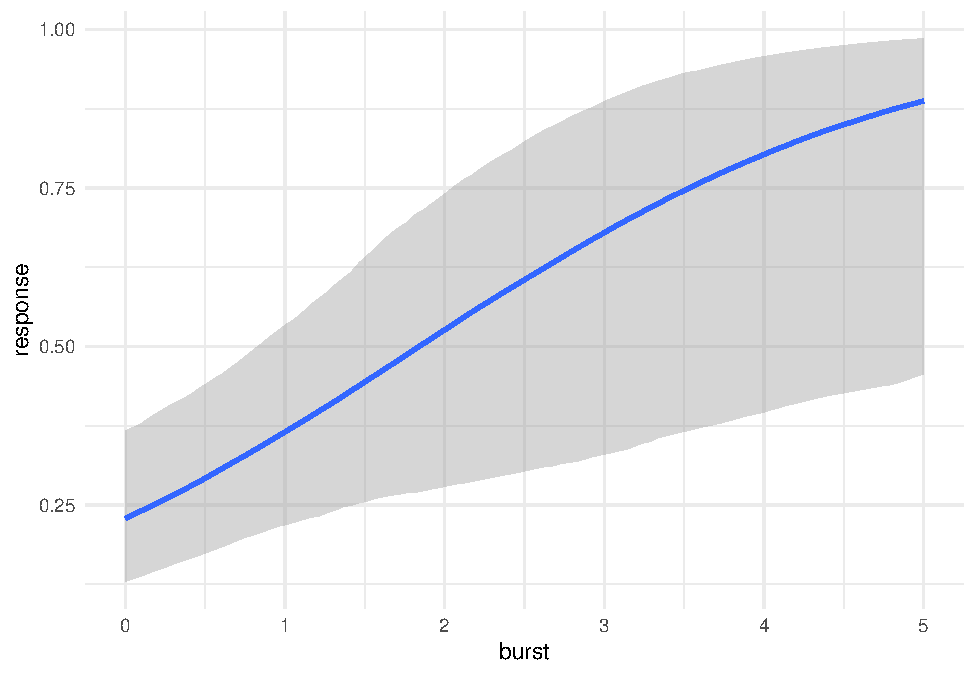
\includegraphics{bayes-reg-3_files/figure-latex/burst-cond-1.pdf}

\begin{Shaded}
\begin{Highlighting}[]
\KeywordTok{conditional\_effects}\NormalTok{(burst\_bm, }\DataTypeTok{spaghetti =} \OtherTok{TRUE}\NormalTok{, }\DataTypeTok{nsamples =} \DecValTok{500}\NormalTok{)}
\end{Highlighting}
\end{Shaded}

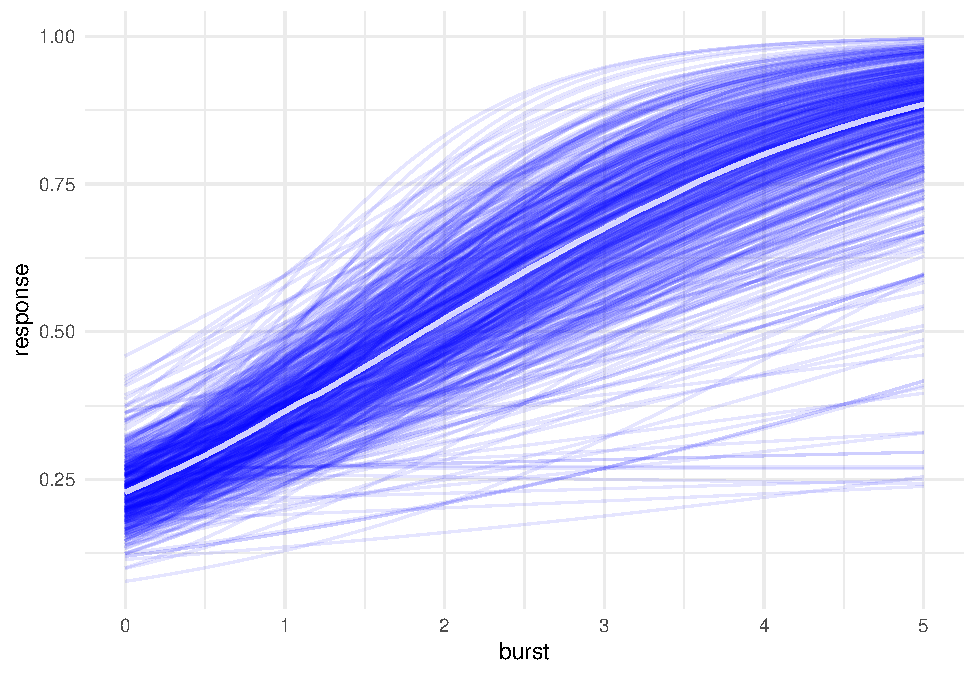
\includegraphics{bayes-reg-3_files/figure-latex/burst-cond-2.pdf}

As you can see, there's a lot of uncertainty (i.e.~large CIs). Not
surprising, given the sample size (which is incredibly small).

\hypertarget{extra}{%
\subsection{Extra}\label{extra}}

Note that a GLMER model with the same random specification as the model
\texttt{burst\_bm} does not converge.

\begin{Shaded}
\begin{Highlighting}[]
\NormalTok{burst\_glm \textless{}{-}}\StringTok{ }\KeywordTok{glmer}\NormalTok{(}
\NormalTok{  response }\OperatorTok{\textasciitilde{}}
\StringTok{    }\NormalTok{burst }\OperatorTok{+}
\StringTok{    }\NormalTok{(burst }\OperatorTok{|}\StringTok{ }\NormalTok{participant),}
  \DataTypeTok{data =}\NormalTok{ burst,}
  \DataTypeTok{family =} \KeywordTok{binomial}\NormalTok{()}
\NormalTok{)}
\end{Highlighting}
\end{Shaded}

\begin{verbatim}
## boundary (singular) fit: see ?isSingular
\end{verbatim}

A simplified model converges and it returns very low \emph{p}-values,
which are clearly anti-conservative values (compare with the high degree
of uncertainty in results of \texttt{burst\_bm}).

\begin{Shaded}
\begin{Highlighting}[]
\NormalTok{burst\_glm\_simple \textless{}{-}}\StringTok{ }\KeywordTok{glmer}\NormalTok{(}
\NormalTok{  response }\OperatorTok{\textasciitilde{}}
\StringTok{    }\NormalTok{burst }\OperatorTok{+}
\StringTok{    }\NormalTok{(}\DecValTok{1} \OperatorTok{|}\StringTok{ }\NormalTok{participant),}
  \DataTypeTok{data =}\NormalTok{ burst,}
  \DataTypeTok{family =} \KeywordTok{binomial}\NormalTok{()}
\NormalTok{)}

\KeywordTok{summary}\NormalTok{(burst\_glm\_simple)}
\end{Highlighting}
\end{Shaded}

\begin{verbatim}
## Generalized linear mixed model fit by maximum likelihood (Laplace
##   Approximation) [glmerMod]
##  Family: binomial  ( logit )
## Formula: response ~ burst + (1 | participant)
##    Data: burst
## 
##      AIC      BIC   logLik deviance df.resid 
##    416.6    428.3   -205.3    410.6      357 
## 
## Scaled residuals: 
##     Min      1Q  Median      3Q     Max 
## -3.1998 -0.7790  0.3703  0.6895  2.3385 
## 
## Random effects:
##  Groups      Name        Variance Std.Dev.
##  participant (Intercept) 0.1516   0.3893  
## Number of obs: 360, groups:  participant, 4
## 
## Fixed effects:
##             Estimate Std. Error z value Pr(>|z|)    
## (Intercept) -1.17930    0.29034  -4.062 4.87e-05 ***
## burst        0.62154    0.07882   7.885 3.14e-15 ***
## ---
## Signif. codes:  0 '***' 0.001 '**' 0.01 '*' 0.05 '.' 0.1 ' ' 1
## 
## Correlation of Fixed Effects:
##       (Intr)
## burst -0.614
\end{verbatim}

\end{document}
